\documentclass{beamer}

\mode<presentation>
\usetheme{Madrid}
\definecolor{Columbia}{RGB}{185,217,235}
\definecolor{Columbia2}{RGB}{0,51,160}
\definecolor{Columbia3}{RGB}{0,114,206}
\setbeamercolor{title}{fg=Columbia2}
\setbeamercolor{frametitle}{fg=Columbia2}
\setbeamercolor{block title}{bg=Columbia, fg=Columbia2}
%\setbeamercolor{block body}{fg=Columbia2}
\setbeamercolor{structure}{fg=Columbia}
\setbeamercolor{item projected}{fg=white}
\setbeamercolor{item}{fg=Columbia2}
\setbeamercolor{subitem}{fg=Columbia2}
\setbeamercolor{section in toc}{fg=Columbia}
\setbeamercolor{description item}{fg=Columbia}
\setbeamercolor{caption name}{fg=Columbia}
\usepackage{graphics}
\usepackage{geometry}
\usepackage{booktabs}
\usepackage{multirow, makecell}
\usepackage{float}
\usepackage{fancyvrb}
\usepackage{caption}
\usepackage{subcaption}
\usepackage{adjustbox}
\usepackage{hyperref}

%\hypersetup{
%colorlinks=true,
%linkcolor=black,
%filecolor=green, 
%urlcolor=blue,
%}
\beamertemplatenavigationsymbolsempty
\setbeamertemplate{footline}[page number]
\setbeamercolor{page number in head/foot}{fg=black}
\setbeamertemplate{headline}{}
\makeatletter
\let\@@magyar@captionfix\relax
\makeatother


\title[Econometrics 2]{Introduction to Econometrics 2: Recitation 11} % Change this regularly
\author{Seung-hun Lee}
\institute{Columbia University}

\date{April 22nd, 2020}

\begin{document}
\begin{frame}
\titlepage
\end{frame}
%%%%%%%%%%%%%%%

\begin{frame}
\frametitle{Failure of Conditional Independence}
When is it violated? 
\begin{itemize}
\item In the regressional framework of $y_{i}(d)=\mu(X_i,d)+\epsilon_i(d)$, the error terms is not independent of $D_i|X_i$.
\item The conditional independence assumption can be broken because:
\begin{itemize}
\item Participants \textbf{self-select based on expected benefit}: In a job training program for plumbing, those who are more healthy are likely to join. If health is not perfectly observed, we risk breaking the conditional independence assumption
\item Participants may be \textbf{selected, consciously or not, to join}: Think of the clinical trial where participation is voluntary. In such case, individuals who are more risk-loving are more likely to join, something not readily observed
\item There may be \textbf{equilibrium effects}: A tuition subsidy program that intends to increase the number of people entering college may have a spillover effect by increasing supply of college graduates at the labor market, leading to a decrease in college premium. This may induce students to enter college less.
\end{itemize}
\end{itemize}
\end{frame}

\begin{frame}
\frametitle{Failure of Conditional Independence}
What happens?
\begin{itemize}
\item Mathematically, what happens is that when we calculate $E[Y_i|D_i=1,x]-E[Y_i|D_i=0,x]$, we end up with
\footnotesize{\begin{align*}
E[Y_i|D_i=1,x]-E[Y_i|D_i=0.x]&=\mu(x.1)-\mu(x,0)+E[\epsilon_i(1)|1,x]-E[\epsilon_i(0)|0,x]\\
&=TE+E[\epsilon_i(1)|1,x]-E[\epsilon_i(0)|0,x]
\end{align*}}\normalsize
\item The error term no longer can be erased from the equation since CIA assumption is not applicable.
\item The difference between the error term is the \textbf{selection bias} (Also appears in Angrist, Pischke 2009). 
\item This also means that the error terms and the $u_i$ in $D_i=1(u_i<p(x_i))$ can covary. The result is that the treatment effect estimated from here can be inaccurate. \par
\item There are two possible solutions. Old method relies on \textbf{Heckman correction}. Recent focus is on IV to derive \textbf{marginal treatment effects} and \textbf{localized average treatment effect}.
\end{itemize}
\end{frame}

\begin{frame}
\frametitle{Failure of Conditional Independence}
Heckman Correction
\begin{itemize}
\item Suppose that we are in the situation where we have a DGP
\[
Y_i = \max\{X_i\beta+\sigma\eta_i, 0\}, \eta_i \sim N(0,1)
\]
So we only see $Y_i$ if $X_i\beta+\sigma\eta_i>0$. We observe $D_i$, specified as
\[
D_i=\begin{cases}1 & \text{if }\eta>-\frac{X_i\beta}{\sigma}\\ 0 & \text{otherwise} \end{cases}
\]
\item Then, for the observed sample, we are likely to have an $\eta_i$ that is positively selected - a nonrandom error leading to a bias
\item The size of the bias is $\frac{\phi(X_i\beta/\sigma)}{\Phi(X_i\beta/\sigma)}=IMR$ (shown in the recitation notes)
\item The $\beta/\sigma$ parameters can be estimated by regressing $D_i$ on $X_i$
\item Include estimated IMR in the observed sample and regress \[
Y_i = X_i\beta+\gamma\hat{f}(x)+\epsilon_i
\]
\end{itemize}
\end{frame}

\begin{frame}
\frametitle{Failure of Conditional Independence}
Instrumental Variables
\begin{itemize}
\item However, Heckman Correction assumes linearity and normality of the error terms.
\item So we look into the UV, where we assume that there exist variables $Z_i$ that affect the treatment $D_i$ but not the outcomes (on its own).
\item It should satisfy
\begin{itemize}
\item \textbf{Relevancy}: It effects the propensity score $p(x,z)=\Pr(D_i=1|X_i=x, Z_i=z)$
\item \textbf{Validity}: Distribution of the counterfactual outcomes and $u_i$ does not depend on $Z_i|X_i$. To put it in mathematical notation, 
\[
(Y_i(1), Y_i(0), u_i) \perp \!\!\!\perp Z_i|X_i
\]
\item \textbf{Full support}: The support of $p(x,z)$ conditional on $x$ extends to all of $[0,1]$. This implies that change in $Z$ induces large variations in the propensity score. 
\end{itemize} 
\end{itemize}
\end{frame}

\begin{frame}
\frametitle{Failure of Conditional Independence}
Identification
\begin{itemize}
\item  So what concerns do we run into in terms of identification? 
\item We can identify $p(x,z)$ by calculating $\Pr(D_i=1|X_i=x, Z_i=z)$. 
\item We can also write
\footnotesize{\begin{align*}
E[Y_i|D_i=1, X_i=x, Z_i=z]&=\mu(x,1)+E[\epsilon_i(1)|u_i<p(x,z), x, z]\\
&=\mu(x,1)+E[\epsilon_i(1)|u_i<p(x,z), x] \ (\because\text{validity})
\end{align*}}\normalsize
\item Define $K_1(p(x,z))=E[\epsilon_i(1)|u_i<p(x,z), X_i=x]$ to be some unknown function of the conditional expectation of $\epsilon_i(1)$. 
\item We can also work similarly to define 
\[
E[Y_i|D_i=0, X_i=x, Z_i=z]=\mu(x,0)+E[\epsilon_i(0)|u_i>p(x,z), X_i=x]
\] 
and $K_0(p(x,z))=E[\epsilon_i(0)|u_i>p(x,z), X_i=x]$
\end{itemize}
\end{frame}

\begin{frame}
\frametitle{Failure of Conditional Independence}
Identification
\begin{itemize}
\item Note that the left hand sides for both sets of equations can be identified by naively taking an average of $Y_i$'s conditional on some the treated (untreated) for the group $X_i=x, Z_i=z$. 
\item The estimated result breaks down into
\[
\mu(x,1)-\mu(x,0)+\underbrace{K_1(p(x,z))-K_0(p(x,z)) }_{\Delta(p(x,z))}= TE(x)+\Delta(p(x,z))
\]
\item $\Delta(p(x,z))$ is the control function that stands for the selection bias.
\item By relevance, change in $z$ affects the value of $p(x,z)$ for a fixed $x$, allowing us to identify how $\Delta(p(x,z))$ \textit{changes}.
\item However, we do not know what the \textit{exact value} of $\Delta(p(x,z))$ is for the initial value of $z$ we started. 
\item Therefore, the true parameter of interest, TE, cannot be uncovered.
\end{itemize}
\end{frame}

\begin{frame}
\frametitle{Failure of Conditional Independence}
Identification
\begin{itemize}
\item So how can we progress on? Note that the $K_d$ functions are conditional expectations of $\epsilon_i(d)$ on $X_i=x$ and selection rule $u_i (<,>) p(x,z)$. 
\item In particular, we can get that
\begin{align*}
K_1(1) &=E[\epsilon_i(1)|u_i<1,X_i=x] \\
&=E[\epsilon_i(1)|X_i=x] \ (\because\text{Everyone is treated})\\
&=0\\
K_0(0) &=E[\epsilon_i(1)|u_i>0,X_i=x] \\
&=E[\epsilon_i(1)|X_i=x] \ (\because\text{No one is treated})\\
&=0
\end{align*}
\item Heckman and Vytlacil show that given a continuous instrument $z$, we can do a much better job of identifying the treatment effect. 
\end{itemize}
\end{frame}

\begin{frame}
\frametitle{Failure of Conditional Independence}
Marginal Treatment Effects
\begin{itemize}
\item The \textbf{marginal treatment effect} at $p(x,z)=p$ is defined as the treatment effect on individuals whose $u_i=p(x,z)$. We can write
\[
MTE(p)=E[Y_i(1)-Y_i(0)| u_i=p]
\]
\item Heckman and Vytlacil show that 
\[
MTE(p)=\frac{\partial E[Y_i | p(x,z)=p]}{\partial p}
\]
\item This is done by 
\begin{enumerate}
\item Estimate $p(x,z)=\Pr(D_i=1|X_i=x. Z_i=z)$
\item Regress $Y_i$ on the estimated $p(x,z)$ in a flexible setting - preferably not just linearly but with some nonlinearities
\item Take a derivative with respect to $p$. (or local linear estimator)
\item For treatment effects, evaluate the $E[Y_i|p(x,z),x]$ at $p(x,z)=1$ and $p(x,z)=0$ and identify the difference. (You can obtain $E[Y_i|\cdot]$ by getting the predicted values).  
\end{enumerate}
\end{itemize}
\end{frame}

\begin{frame}
\frametitle{Failure of Conditional Independence}
Marginal Treatment Effects
\begin{itemize}
\item Intuitively, what is going on with MTE is as follows
\item By changing $p$ slightly by $dp$, we are able to identify the marginal compliers who move from not being treated to being treated. 
\item We are finding out how their outcome changes as they move from non-participation to participation into the treatment
\end{itemize}
Math Behind MTE
\begin{itemize}
\item Define
\[
G(p)=E[Y_i\cdot 1(p(x,z)=p)]
\]
\item \footnotesize{$Y_i=D_iY_i(1)+(1-D_i)Y_i(0)=1(u_i<p(x,z))Y_i(1)+1(u_i>p(x,z))Y_i(0)$}\normalsize, so we can rewrite the above as
\footnotesize{\begin{align*}
G(p)&=E[Y_i(1)\cdot 1(u_i<p)\cdot 1(p(x,z)=p)]+E[Y_i(0)\cdot 1(u_i>p)\cdot 1(p(x,z)=p)]\\
&=G_1(p)+G_0(p)
\end{align*}}\normalsize
\end{itemize}
\end{frame}

\begin{frame}
\frametitle{Failure of Conditional Independence}
Math Behind MTE
\begin{itemize}
\item By the validity condition and the fact that $u_i\sim U[0,1]$ (and thus $f(u_i)=1$), we can write
\footnotesize{\begin{align*}
E[Y_i(1)\cdot 1(u_i<p)\cdot 1(p(x,z)=p)]&=E[Y_i(1)\cdot 1(u_i<p)]\Pr(p(x,z)=p)\\
&=\int_0^pE[Y_i(1)|u=t]dt\Pr(p(x,z)=p)
\end{align*}}\normalsize
And similarly, 
\footnotesize{\[
E[Y_i(0)\cdot 1(u_i>p)\cdot 1(p(x,z)=p)]=\int_p^1E[Y_i(0)|u=t]dt\Pr(p(x,z)=p)
\]}\normalsize
\item So 
\footnotesize{\[
G(p)=\left(\int_0^pE[Y_i(1)|u=t]dt+\int_p^1E[Y_i(0)|u=t]dt\right)\Pr(p(x,z)=p)
\]}\normalsize
\end{itemize}
\end{frame}

\begin{frame}
\frametitle{Failure of Conditional Independence}
Math Behind MTE
\begin{itemize}
\item Since $E[Y_i\cdot 1(p(x,z)=p)]=E[Y_i|p(x,z)=p]\cdot \Pr(p(x,z)=p) $ this implies that
\footnotesize{\[
E[Y_i|p(x,z)=p]=\frac{G(p)}{\Pr(p(x,z)=p)}=\int_0^pE[Y_i(1)|u=t]dt+\int_p^1E[Y_i(0)|u=t]dt
\]}\normalsize
\item Then, by Leibniz's integral rule
\[
\frac{\partial E[Y_i | p(x,z)=p]}{\partial p}=E[Y_i(1)|u=p]-E[Y_i(0)|u=p]=MTE(p)
\]
\item Hence, the treatment effect can be recovered by
\[
TE=\int_0^1MTE(p)dp=E[Y_i|p(x,z)=1]-E[Y_i|p(x,z)=0]
\]
\end{itemize}
\end{frame}

\begin{frame}
\frametitle{Failure of Conditional Independence}
Some Caveats with MTE
\begin{itemize}
\item For the above methods to work, we need the $Z_i$ instruments to satisfy
\begin{itemize}
\item $Z$ belongs in the treatment (relevancy): $D_i=1(u_i<p(X_i,Z_i))$
\item $Z$ not belong in the outcome (exclusivity): $Y_i(d)=\mu(x,d)+\epsilon_i(d)$
\item In other words, we get $(\epsilon_i(1), \epsilon_i(0), u_i) \perp\!\!\!\perp Z_i|X_i$
\item Continuity: $p(x,z)$ changes w.r.t $z$ in a continuous way (This is because we need to be able to take derivatives)
\end{itemize}
\item For the range of $p(x,z)$ available, the above condition allows us to estimate the marginal treatment effect. 
\item For any work you see that uses marginal treatment effect, there includes a graph that maps marginal treatment effect on the vertical axis and the `resistance' parameter $u_i$ on the horizontal axis.
\end{itemize}
\end{frame}

\begin{frame}
\frametitle{Failure of Conditional Independence}
Testing CIA
\begin{itemize}
\item With this framework, we can also test if conditional independence assumption holds. 
\item Recall that conditional independence assumption is satisfied when
\[
(\epsilon_i(1),\epsilon_i(0)) \perp\!\!\!\perp u_i|X_i
\]
\item In cases where this is true, then the outcomes are independent of $u_i$ conditional on $X_i$. Thus, 
\[
MTE(x,p)=E[Y_i(1)-Y_i(0)|X_i=x, u_i=p]=E[Y_i(1)-Y_i(0)|X_i=x]
\]
\item Since $MTE(x,p)=\frac{\partial E[Y_i | X_i=x, p(x, z)=p]}{\partial p}$, the above condition implies that $E[Y_i|X_i=x, p(x, z)=p]$ is linear in $p$. 
\item Thus, it is highly recommended to put polynomial terms of $p^k, k=1,2,3,...$ when you estimate marginal treatment effects. \item Then, test to find whether the nonlinear terms have coefficient zero. 
\end{itemize}
\end{frame}

\begin{frame}
\frametitle{Failure of Conditional Independence}
Examples 
\begin{itemize}
\item Carneiro, Lee (2009): The paper estimates the impact of attending college on log wage distributions. The paper finds that individuals more likely to attend college (and have low resistance parameters) are more likely to have higher college wage ($Y_i(1)$) over high school wage ($Y_i(0)$). The opposite holds true for people with high school degree. They have a MTE figure (at figure 3) that maps MTE as a function of resistance parameters.
\item Johnson, Taylor (2019): The paper shows that causal impact of migration decreases longevity (at least heterogenously). This is even with the consideration that migrants are more likely to be educated and have higher baseline earnings compared to non-migrants. They use the MTE to (with railcar traffic at the town of origin as one of their IVs). They document that those who have lower latent ability (high $U_d$) suffer more from migrating out, reflected in the downward sloping MTE 
\end{itemize}
\end{frame}

\begin{frame}
\frametitle{Failure of Conditional Independence}
\centering
\begin{figure}[H]
\begin{subfigure}{0.45\textwidth}
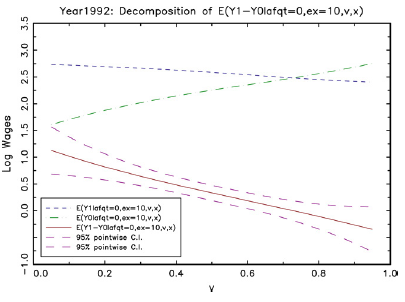
\includegraphics[width=\textwidth]{fig11_1}
\caption{Carneiro, Lee (2009)}
\end{subfigure}
\begin{subfigure}{0.45\textwidth}
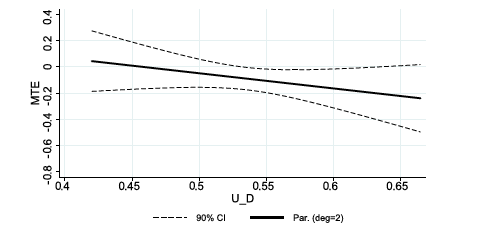
\includegraphics[width=\textwidth]{fig11_2}
\caption{Johnson, Taylor (2019)}
\end{subfigure}
\end{figure}
\end{frame}

\begin{frame}
\frametitle{Failure of Conditional Independence}
Local Average Treatment Effect
\begin{itemize}
\item The marginal treatment effect looks at `marginal' compliers: It is interested in the small group of individuals who changes treatment status from $D_i=0$  to $D_i=1$ as $p(x,z)$ changes slightly due to $Z_i$
\item Instead of changing the propensity score by a tiny bit, we can look at finite differences - like $Z_i$ having just two possible values. 
\item Then we are going to be looking at a larger group of compliers than in the marginal treatment effect context. The treatment effect for this larger group of compliers is called \textbf{local average treatment effect}.
\item We will setup the framework as follows:
\begin{itemize}
\item $Z_i$ will be a binary instrumental variable. This of this as eligibility rule. 
\item $D_i(z)$ can be characterized as $D_i(z)=1(u_i<p(x,z))$. Note that as $z$ rises, so will $p(x,z)$. This is the relevance condition
\item $Z_i$ itself has no bearing, at least directly, on the outcome. So $Y_i(d)=\mu(x,d)+\epsilon_i(d)$. So we still have $(\epsilon_i(1), \epsilon_i(0), u_i)\perp\!\!\!\perp Z_i|X_i$. 
\end{itemize}
\end{itemize}
\end{frame}

\begin{frame}
\frametitle{Failure of Conditional Independence}
Local Average Treatment Effect
\begin{itemize}
\item The formal way to define local average treatment effect is as follows
\[
LATE(x)=E[Y_i(1)-Y_i(0)|p(x,z)<u_i<p(x,z'). X_i=x]
\]
\item We can identify LATE by using the following (I skip $X_i=x$)
\footnotesize{\begin{align*}
E[Y_i|Z_i=z']-E[Y_i|Z_i=z]&=E[1(u_i<p(z'))Y_i(1)+1(u_i>p(z'))Y_i(0)|z']\\
&-E[1(u_i<p(z))Y_i(1)+1(u_i>p(z))Y_i(0)|z]\\
&=E[1(u_i<p(z'))Y_i(1)+1(u_i>p(z'))Y_i(0)]\\
&-E[1(u_i<p(z))Y_i(1)+1(u_i>p(z))Y_i(0)]\\
&=E[(1(u_i<p(z'))-1(u_i<p(z))Y_i(1)\\
&-(1(u_i>p(z'))-1(u_i>p(z))Y_i(0)]\\
&=E[(1(u_i<p(z'))-1(u_i<p(z))(Y_i(1)-Y_i(0))]\\
&=\Pr[1(u_i<p(z'))-1(u_i<p(z))=1]\\
&\times E[Y_i(1)-Y_i(0)|1(u_i<p(z'))-1(u_i<p(z))=1]
\end{align*}}\normalsize
\end{itemize}
\end{frame}

\begin{frame}
\frametitle{Failure of Conditional Independence}
Local Average Treatment Effect
\begin{itemize}
\item We only consider complies and $1(u_i<p(z'))-1(u_i<p(z))=1$ holds iff $p(z)<u_i<p(z')$. 
 \footnotesize{\begin{align*}
E[Y_i|z']-E[Y_i|z]&=\Pr[p(z)<u_i<p(z')]E[Y_i(1)-Y_i(0)|p(z)<u_i<p(z')]
\end{align*}}\normalsize
\item Therefore, we are able to identify LATE as
\footnotesize{\[
LATE(x, z,z')=\frac{E[Y_i|Z_i=z']-E[Y_i|Z_i=z]}{\Pr(p(z)<u_i<p(z'))}=\frac{E[Y_i|Z_i=z']-E[Y_i|Z_i=z]}{p(z')-p(z)}
\]}\normalsize
\item Or in terms of the propensity score (and by bringing $X_i=x$ back in)
\[
LATE(x, p(z),p(z'))=\frac{E[Y_i|p=p(x.z')]-E[Y_i|p=p(x,z)]}{p(x,z')-p(x,z)}
\]
\end{itemize}
\end{frame}

\begin{frame}
\frametitle{Failure of Conditional Independence}
Local Average Treatment Effect
\begin{itemize}

\item We can go further: Estimate propensity scores with
\[
p(x,z)=E[D_i|X_i=x, Z_i=z]
\]
and get
\[
LATE(x, z,z')=\frac{E[Y_i|x,z']-E[Y_i|x,z]}{E[D_i|x,z']-E[D_i|x,z]}
\]
\item To obtain this from the regression, we follow these steps:
\begin{enumerate}
\item Regress $D$ on $Z$ and other covariates $X$ to get $\hat{D}=\hat{p}(x,z)$
\item Regress $Y$ on other covariates $X$ and $\hat{D}$.
\end{enumerate}
The LATE estimator can then be obtained here is called the Wald estimator. 
\end{itemize}
\end{frame}

\begin{frame}
\frametitle{Failure of Conditional Independence}
Some Words on Monotonicity Condition
\begin{itemize}
\item When we wrote $D_i=1(u_i<p(x,z))$ and assume that $P(x,z)$ rises with $z$ for fixed $x$, monotonicity condition implies that $D_i$ can only increase.
\item We are ruling out a case where $D_i$ can change from 1 to 0. (Defiers)
\item We also throw away information on the always takers and never takers as well. 
\item Both LATE and MTE can only tells us about compliers while throwing away defiers. 
\item This condition, along with the validity condition, cannot be tested empirically.  Therefore, the applicability of this condition should be argued using intuition or external facts. 
\end{itemize}
\end{frame}
%%%%%%%%%%%
\end{document}
